% The projective-plane boundary complex before and after reduction modulo two.
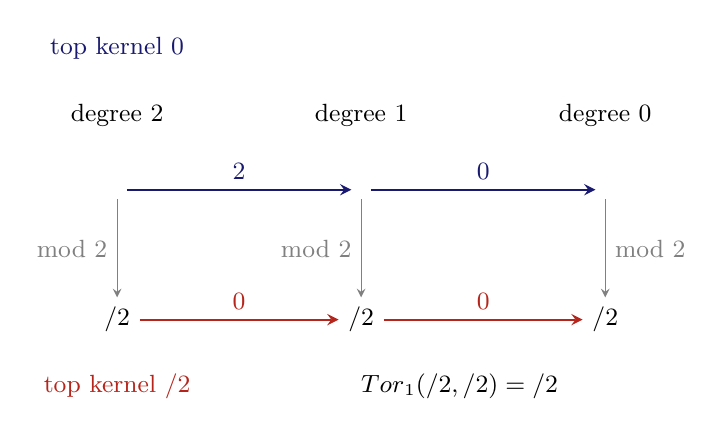
\begin{tikzpicture}[font=\small,>=stealth,x=1cm,y=1cm]
\node at (0,2.6) {degree $2$};
\node at (3.1,2.6) {degree $1$};
\node at (6.2,2.6) {degree $0$};
\node (z2) at (0,1.65) {$\Z$};
\node (z1) at (3.1,1.65) {$\Z$};
\node (z0) at (6.2,1.65) {$\Z$};
\draw[->,thick,MidnightBlue] (z2) -- node[above] {$2$} (z1);
\draw[->,thick,MidnightBlue] (z1) -- node[above] {$0$} (z0);
\node (f2) at (0,0) {$\Z/2$};
\node (f1) at (3.1,0) {$\Z/2$};
\node (f0) at (6.2,0) {$\Z/2$};
\draw[->,thick,BrickRed] (f2) -- node[above] {$0$} (f1);
\draw[->,thick,BrickRed] (f1) -- node[above] {$0$} (f0);
\draw[->,gray] (z2) -- node[left] {mod $2$} (f2);
\draw[->,gray] (z1) -- node[left] {mod $2$} (f1);
\draw[->,gray] (z0) -- node[right] {mod $2$} (f0);
\node[align=center,MidnightBlue] at (0,3.45) {top kernel $0$};
\node[align=center,BrickRed] at (0,-0.85) {top kernel $\Z/2$};
\node[align=center] at (4.35,-0.85) {$\operatorname{Tor}_1(\Z/2,\Z/2)=\Z/2$};
\end{tikzpicture}
